\chapter{London dispersion}
\label{ch:t-dispersion}
\index{London dispersion}
\index{Argon dimer}
\index{Intermolecular interactions}
\eccexample{Examples > General Chemistry > Intermolecular interactions}

Two argon atoms carry no charge and no dipole, and their electron shells are closed, yet argon condenses when it is cold enough, so something must hold the atoms together. The attraction is London dispersion: the electron clouds of the two atoms fluctuate, and the fluctuations in one atom are correlated with those in the other, so that the pair is on average a little lower in energy close together than far apart. This chapter gives the teacher one curve, the energy of two argon atoms against their distance, to show a class that this attraction exists, how weak it is next to a hydrogen bond, and why it still matters. The argon dimer is the cleanest case to show, since nothing else contributes.

\section*{This requires}
Nothing beyond ECCE: the calculation is in the General Chemistry example set.

\section{The calculation}
The topic \menu{Intermolecular interactions} holds the argon dimer \emph{ar\_dimer}, optimised in ECCE in the same way as the water dimer of Chapter~\ref{sec:hydrogen-bond}. For the curve of figure~\ref{fig:disp-curve} the Ar--Ar distance was scanned (Chapter~\ref{ch:scans}), from \SI{0.4}{\angstrom} inside the optimised distance out to \SI{10}{\angstrom}. Each point is the energy of the pair relative to two argon atoms calculated separately, in kJ/mol, the energy per mole of pairs; a negative value means that the pair is held together by that much energy.

\section{The curve}
The curve shows how deep the attraction is and how it changes with distance. Its lowest point is at \SI{3.78}{\angstrom}, only \SI{1.2}{kJ.mol^{-1}} below two separate argon atoms (table~\ref{tab:disp-curve}). Spectroscopy of argon dimers in the gas phase puts the bottom of the real well at \SI{3.76}{\angstrom} and \SI{1.19}{kJ.mol^{-1}} (99.2~cm$^{-1}$) below the separate atoms \cite{herman1988}, so the calculated curve has both the position and the depth of the measured one. The two sides of the well are very different: moving the atoms \SI{0.4}{\angstrom} closer than the minimum raises the energy by \SI{1.3}{kJ.mol^{-1}}, more than the whole depth of the well, while moving them \SI{0.4}{\angstrom} apart costs only \SI{0.3}{kJ.mol^{-1}}. The steep inner wall is the repulsion of the two closed shells, which sets in abruptly once they touch, and the shallow outer side is the dispersion attraction, which dies away slowly with distance. Hence the curve shows both halves of the familiar picture of atoms as soft spheres, a hard core with a weak, long attractive tail. Beyond about \SI{8}{\angstrom} the points scatter by a few hundredths of a kJ/mol around zero; that is the numerical precision of the calculation, not a feature of the attraction.

\begin{figure}[htbp]
	\centering
	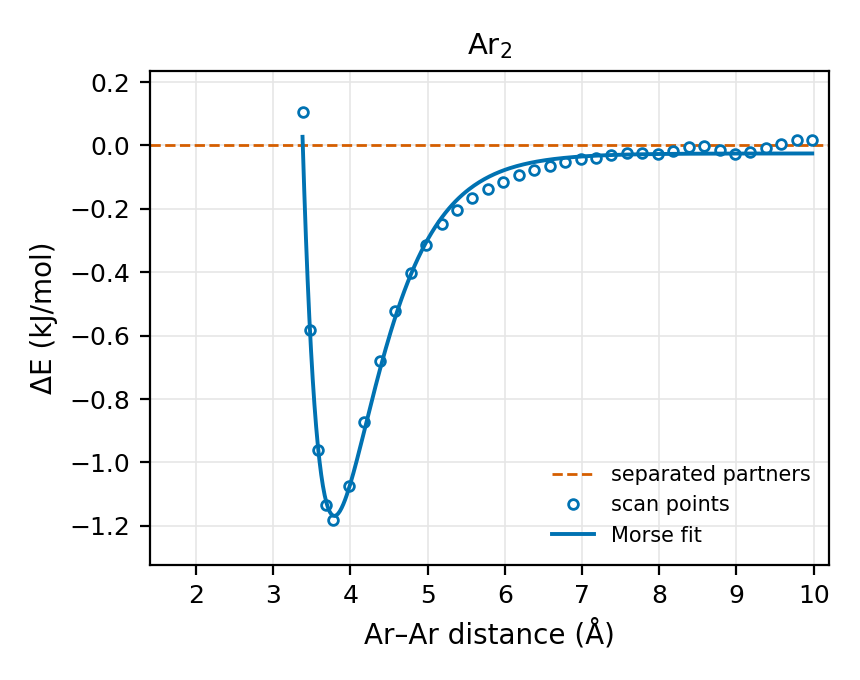
\includegraphics[width=0.6\linewidth]{dispersion/dispersion-curve.ecce-9.5.3-dev.png}
	\caption{Energy of the argon dimer against the Ar--Ar distance, from a relaxed scan in ECCE. Zero (dashed) is two argon atoms calculated separately. Note the energy scale, about twenty times smaller than that of the water dimer in figure~\ref{fig:hb-curve}.}
	\label{fig:disp-curve}
\end{figure}

\begin{table}[htbp]
	\centering
	\caption{The curve of figure~\ref{fig:disp-curve}. $\Delta E_\mathrm{min}$ is the lowest point, at the distance $R_\mathrm{min}$, and $\Delta E(R_\mathrm{max})$ the point at the largest distance $R_\mathrm{max}$, both relative to two separate argon atoms. Energies in kJ/mol.}
	\label{tab:disp-curve}
	\begin{tabular}{rrrr}
		\toprule
		$R_\mathrm{min}$ (\AA) & $\Delta E_\mathrm{min}$ & $\Delta E(R_\mathrm{max})$ & $R_\mathrm{max}$ (\AA) \\
		\midrule
		3.78 & $-1.2$ & 0.0 & 9.98 \\
		\bottomrule
	\end{tabular}
\end{table}

The comparison with the hydrogen bond puts the depth in proportion. The water dimer, scanned in the same way, is \SI{25.9}{kJ.mol^{-1}} deep (Chapter~\ref{sec:hydrogen-bond}), about twenty times deeper than the argon well. At room temperature $RT$, the typical energy that molecules exchange in collisions, is \SI{2.5}{kJ.mol^{-1}}, twice the depth of the argon well, so collisions break an argon pair apart almost as soon as it forms. Hence argon is a gas at room temperature and becomes a liquid only when it is cooled far enough for collisions to be gentle compared with the depth of the well. Argon boils at \SI{87.3}{K} (\SI{-185.9}{\celsius}) \cite{gosman1969}, where $RT$ is \SI{0.73}{kJ.mol^{-1}}, less than the depth of the well.
\index{Relaxed scan!interaction curves}

\section{Non-covalent interactions}
The \menu{NCI} surface (\menu{Properties > Orbitals > Surfaces}, \menu{NCI}), described with the water dimer in Chapter~\ref{sec:hydrogen-bond}, shows the contact between the two argon atoms in the same way. ECCE draws it only where the electron density is low and changes slowly, and colours it on one fixed scale: blue for an attraction with density gathered between two atoms, as in a hydrogen bond, green for a weak contact with very little density, and red for atoms crowded too close. In the argon dimer at its minimum the only surface is a single disc halfway between the two atoms, across the line joining them, and it is green (figure~\ref{fig:disp-nci}).

This figure shows that the two atoms meet in a contact with very little electron density, because green is the colour the fixed scale gives where the density between the atoms is close to zero. Hence we can see that the argon atoms are only touching, held by the weak attraction of the shallow well in figure~\ref{fig:disp-curve}, and not by an attraction with density gathered between them as in a hydrogen bond.
\index{NCI}

\begin{figure}[htbp]
	\centering
	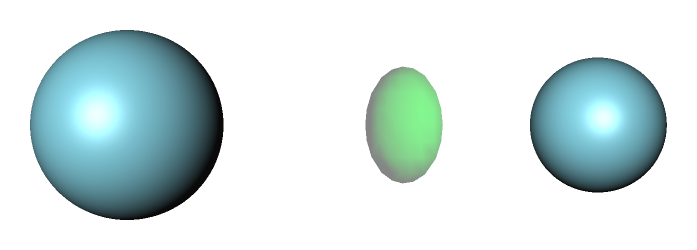
\includegraphics[width=0.6\linewidth]{dispersion/nci.ecce-9.5.3-dev.png}
	\caption{NCI surface of the argon dimer at its minimum (\menu{Properties > Orbitals > Surfaces}, \menu{NCI}). The only surface is the disc halfway between the two atoms. Its colour tells the kind of contact on a fixed scale: blue attraction, as in a hydrogen bond; green a weak contact with little density; red repulsion. The disc is green. The molecule is turned so that the disc shows; the left atom is nearer the viewer and looks larger.}
	\label{fig:disp-nci}
\end{figure}

\section{Three contacts side by side}
The NCI surfaces of three chapters set side by side (figure~\ref{fig:disp-nci-three}) give a class the kinds of contact in one picture: the argon dimer of this chapter, the water dimer of Chapter~\ref{sec:hydrogen-bond} and Na$^+\cdots$H$_2$O of Chapter~\ref{ch:t-ion-dipole}. Each has one disc between the partners. The argon disc is green, while the discs of the hydrogen bond and of the ion--water contact are both pale blue and look much alike, so the colour separates a weak dispersion contact from an attraction with density between the partners, but not a hydrogen bond from an ion--dipole contact; their strengths are told apart by the energies of the curves. None of the three shows red, since at the optimised distance no atoms are pushed together too closely.

This figure shows that dispersion is a different kind of contact from the hydrogen bond and the ion--dipole attraction, because the same fixed colour scale makes the argon disc green and the other two blue. Hence we can see in one picture that argon atoms are held by a weaker kind of contact than the one that holds two water molecules together or a water molecule to a dissolved ion.

\begin{figure}[htbp]
	\centering
	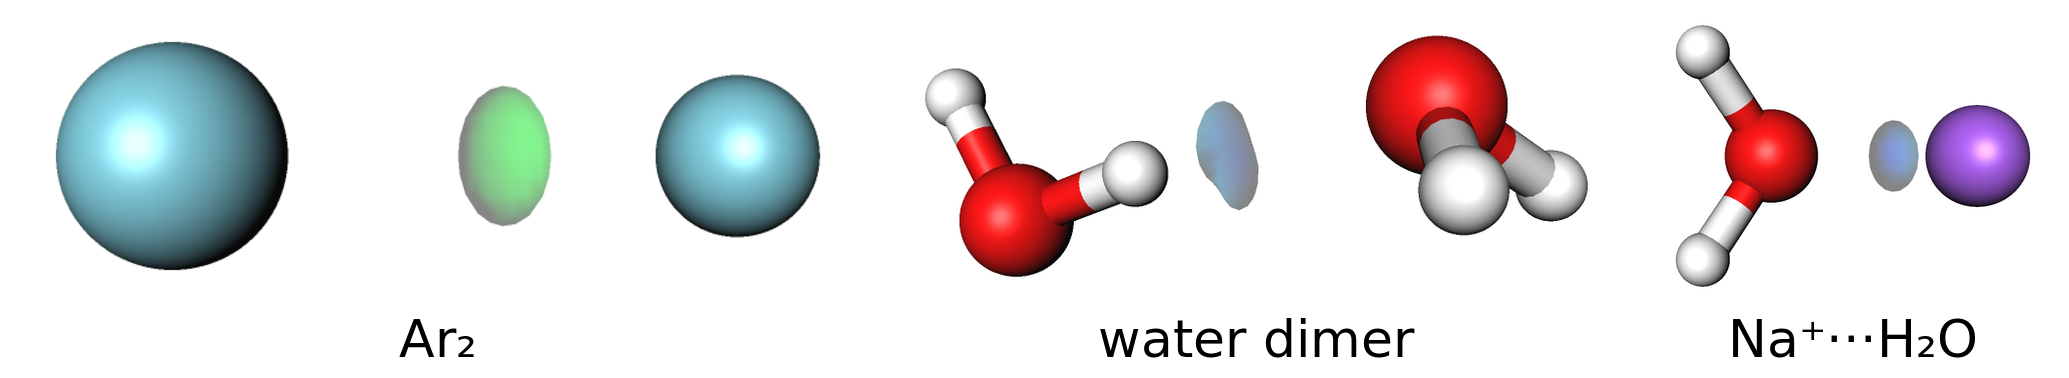
\includegraphics[width=\linewidth]{dispersion/nci-three.ecce-9.5.3-dev.png}
	\caption{NCI surfaces of the argon dimer (left, figure~\ref{fig:disp-nci}), the water dimer (middle, figure~\ref{fig:hb-nci}) and Na$^+\cdots$H$_2$O (right, figure~\ref{fig:id-nci}), each at its optimised structure, on the same fixed colour scale: blue attraction, green a weak contact with little density, red repulsion. The argon disc is green, the other two are blue; the surfaces are drawn partly transparent, which makes the blue look pale on a white background.}
	\label{fig:disp-nci-three}
\end{figure}

\section{In class}
Start with the question why argon, with no charges, no dipoles and full shells, becomes a liquid at all, and then show figure~\ref{fig:disp-curve} with its numbers next to those of the water dimer. Figure~\ref{fig:disp-nci-three} then shows the difference in colour: green for argon, blue for the hydrogen bond and for the ion next to a water molecule. The attraction between two single atoms is weak, but dispersion acts between every pair of atoms in contact, so it adds up for large molecules; this is why the boiling points of the straight-chain alkanes rise with chain length.

\section{History}
Van der Waals gave real gases an attraction between their molecules in his thesis of 1873, as the constant $a$ of his equation of state, without saying where the attraction came from \cite{vanderwaals1873}. Debye in 1920 and Keesom in 1921 traced it to the electric moments of the molecules: a permanent dipole or quadrupole induces a dipole in its neighbour (Debye), and permanent moments that rotate attract each other on average (Keesom) \cite{debye1920,keesom1921}. Neither mechanism applies to atoms of the noble gases, which have no permanent moments, and yet argon condenses. Jones (later Lennard-Jones) fitted an intermolecular potential with an attractive and a repulsive power of the distance to the equation of state of argon in 1924 \cite{jones1924}, and in 1931 settled on the form with $R^{-6}$ attraction and $R^{-12}$ repulsion that carries his name \cite{lennardjones1931}.
\index{van der Waals, Johannes Diderik}\index{Debye, Peter}\index{Keesom, Willem Hendrik}\index{Lennard-Jones, John}

The $R^{-6}$ attraction itself was explained by quantum mechanics. Eisenschitz and London calculated it for two hydrogen atoms in 1930, and London gave the general treatment the same year: the momentary dipoles of the two electron distributions are correlated, which lowers the energy of the pair by an amount that falls off as $R^{-6}$ \cite{eisenschitz1930,london1930}. London called the effect dispersion, after its connection with the optical dispersion of the atoms, and his 1937 paper in the Transactions of the Faraday Society gave the theory in English \cite{london1937}.
\index{London, Fritz}\index{Eisenschitz, Robert}
